\documentclass[a4paper, 11pt]{article}

%-------------------------------------------------------------------------------
%--- (a) Required Packages
%-------------------------------------------------------------------------------
\usepackage{amsmath,amsfonts,amssymb,amsthm}
\usepackage{authblk}
\usepackage[english]{babel}
\usepackage[para,online,flushleft]{threeparttable}
\usepackage{booktabs}
\usepackage{caption}
\usepackage[usenames, dvipsnames]{color}
\usepackage{epstopdf}
\usepackage[capposition=top]{floatrow}
\usepackage{framed}
\usepackage[T1]{fontenc}
\usepackage{graphicx}
\usepackage{hyperref}
\usepackage[utf8]{inputenc}
\usepackage{lscape}
\usepackage{multirow}
\usepackage{natbib}
\usepackage{setspace}
\usepackage{rotating}
\usepackage{subcaption}
\usepackage{subfloat}
\usepackage{url}
\usepackage{wrapfig}
 \usepackage{multicol}
\usepackage[toc,page]{appendix}
%-------------------------------------------------------------------------------
%--- (b) Specific margins
%-------------------------------------------------------------------------------
\setlength  \textwidth{\paperwidth}
\setlength  \textheight{\paperheight}
\setlength  \oddsidemargin{3cm}
\setlength  \topmargin{-1.2cm}
\setlength  \footnotesep{2ex}
\addtolength\textheight{-6cm}
\addtolength\textwidth{-6cm}
\addtolength\oddsidemargin{-1in}



%-------------------------------------------------------------------------------
%--- (c) Internal Ref stype
%-------------------------------------------------------------------------------
\hypersetup{                                                                                                   
    colorlinks=true,   
    linkcolor=BlueViolet,
    citecolor=BlueViolet,
    filecolor=BlueViolet,
    urlcolor=BlueViolet
}


%-------------------------------------------------------------------------------
%--- (1) Title
%-------------------------------------------------------------------------------
\title{The Effect of Legalised Induced Abortion on Births and Maternal Deaths: 
A Population Based Cohort Study from Mexico}

\author[1]{Damian Clarke}
\author[2]{Hanna Mühlrad}


\affil[2]{University of Gothenburg \\
  \url{hanna.muhlrad@gu.se}}
\affil[1]{University of Oxford \\
  \url{damian.clarke@economics.ox.ac.uk}}


%-------------------------------------------------------------------------------
%--- (2) Document
%---     Notes: Abstract file follows requested 'extended abstract' style of the
%---     BMJ.  Discussion section also follows the BMJ's in house style. A quick
%---     notes box is added at the end of the document in-line with original ar-
%---     ticle requirements for the BMJ.
%-------------------------------------------------------------------------------
\begin{document}
\begin{spacing}{1.25}


\maketitle
\begin{abstract}
\noindent \textbf{Objective:} To determine the effect of access to safe, legal 
abortion on rates of birth, and rates of maternal death.\\
\textbf{Design:} Population based cohort study. \\
\textbf{Setting and participants:} 23,151,080 live births and 11,885 maternal 
deaths in Mexico from 2002 to 2011. \\
\textbf{Interventions:} The decriminalization of induced abortion in Mexico City 
(Federal District) in April 2007, with legal access to free first-term abortions
for all resident women. \\
\textbf{Main outcome measures:} Variation in the rates of births and maternal 
deaths in abortion and non-abortion states following an abortion reform in Mexico 
in 2007.  Prevailing differences prior to the reform are captured using state 
controls, and controls are included for concurrent potentially confouding 
variables including access to hospitals, contraceptives, and other social 
reforms.\\
\textbf{Results:} Safe, legal and free abortion was granted to 8.03\% of Mexico's
female population.  Among fertile-aged covered women, access to abortion (during 
the first 12 weeks of gestation) resulted in reductions in birth rates (2.32 per 
1,000 women; 95\% confidence interval of \textcolor{red}{x.xx-x.xx}) and the 
maternal mortality ratio (13.22 per 100,000 live births; 
\textcolor{red}{x.xx-x.xx}) when compared with uncovered women over the same 
time period and adjusting for confouding factors. \\
\textbf{Conclusions:} Decriminalization and access to safe legal abortions in 
circumstances where clandestine abortion is frequently practiced can lead to 
important reductions in maternal deaths related to childbirth and reduce births
rates due to undesired childbearing, particularly among younger and older women.
\end{abstract}

 
\end{spacing}
\begin{spacing}{1.5}
 
 
%-------------------------------------------------------------------------------
%--- (3) Document
%---    Notes: I'm copying the sections and subsections for the BMJ article 
%---	  "Maternal overweight and obesity in early pregnancy
%---    and risk of infant mortality: a population based cohort study in Sweden"
%-------------------------------------------------------------------------------
\newpage
\begin{multicols}{2}
\section{Introduction}
Unintended pregnancy and lack of access to family planning result in an 
estimated 22 million unsafe abortions world-wide every year.  It is estimated 
that these procedures account for 13 percent of all maternal deaths 
(\textcolor{red}{This citation needs to be added to the bibliography} WHO, 2014).  
Despite increasing attention being paid to rates of morbidity and mortality 
following unsafe abortion procedures \citep{Grimes2006,Brown2007,Kulczycki2011}, 
adequately measuring the impacts of access (or lack thereof) to safe abortion is 
often hindered by poor and incomplete vital registration systems, and a paucity of 
appropriate (quasi-)experimental variation in access to safe abortion 
\citep{Grimes2006}.


----------------------------------------------------------------------------------
 
 In this paper, we examine the 2007 abortion reform in Mexico City. Abortion laws in Mexico are determined at state level where Mexico City (or the Federal District), the administrative capital and a region of Mexico, is the only district out of Mexico's 32 districts that allows for elective abortion during the first trimester. This reform provided all women, with residency in Mexico City and above age 18, with access to legal and safe abortion procedures free of charge during the first trimester for all reasons. The reform was a radical change from previous laws which banned abortion in all but extreme circumstances of rape, to save the mother’s life, or in the case of fetal malformation. 

Important numbers: \citet{Sedghetal2007,Sedghetal2012,Khanetal2006}.
Important discussion: \citet{WinikoffSheldon2012,TheLancet2009,TheLancet2007,Chowdhury2007}. 
Interesting, but probably unrelated: \citet{TempletonGrimes2011}

 By using the 2007 abortion reform in Mexico City, we study the effect of accessing legal and safe abortion services free of charge on fertility outcomes and maternal mortality. This analysis is carried out using Mexican censal data from National Institute of Statistics and Geography (INEGI) on all registered births and maternal deaths during 2002-2011. We use a quasi-experimental set up, since abortion laws are determined at state level providing sub-national variation, employing a difference in difference design to determine the effect of the reform. The results indicate that a drop in the birth rate of 1.7-2.7 births per 1000 women in fertile ages 15-44 can be attributed to the abortion reform. Analyzing heterogeneous effects across age groups, we find that the drop in birth rates is the highest amongst teenage women (15-24) and women aged 34-39. Moreover, we find that access to legal and safe abortion decreases maternal mortality ratio by 9.93-11.63 maternal deaths per 100 000 live births. Heterogeneity analysis shows that this effect is driven by ages 20-34. 
 
 Our results suggest that legalizing elective abortion is potentially important for preventing unwanted pregnancies and maternal mortality. This result is highly relevant for meeting the Millennium Development Goals (MDG) 5 of improved maternal health globally. The fact that the results indicate that access to legal and safe abortions have a positive effect on maternal and reproductive health in Mexico City, the most urban and developed region of Mexico, implies that more rural and poor areas could benefit greatly from a similar reform.        
 \subsection{Background}
 With regards to the highly conservative abortion legislation in the entire Latin American and Caribbean (LAC) region, the abortion reform in Mexico City is distinguishable as a major social and political reform. Abortions are not only illegal but also a criminal offense in many Mexican districts. In several Mexican districts, women suffering from miscarriages are at risk of being prosecuted and sentenced to jail for not protecting their fetus. Before the reform was passed in Mexico City, abortion laws were rather uniform across the districts of Mexico.  Abortion was illegal with the exception of pregnancies resulting from rape, or pregnancies that pose a threat to the mother's life and for some states, in case of severe malformation. In practice however, legal abortions have been described by human rights organizations as extremely difficult to access due to rigid legal barriers even for women who do met the prerequisite for accessing legal abortion. Legal barriers that cause protracted processes, usually involving multiple governmental entities to review the decision, in addition to social stigma explains the low number of legal abortion prior the reform. For an example, in the densely populated Mexico City, only 62 abortions were legally performed during 2001-2007 due to these circumstances,  \cite{Becker,Madrazo2009,Levinetal2009,Schiavonetal2010,JuarezSingh2012}. 
 
 As a substitute to legal options, abortions are made under clandestine and not unusually unsafe settings. In 2009 alone, records from public hospitals show that an estimated 159 000 women were treated for abortion-related complications. Moreover, the estimated national abortion rate in Mexico is 38 abortions per 1000 women in the ages 15-44 (GIRE, 2009), which is considered high internationally \cite{Becker}. Due to the high number of unsafe abortions as well as a growing movement for women's reproductive health rights, a new reform came about legalizing abortion in Mexico City, enabling women to terminate the pregnancy during the first trimester\footnote{For a broader discussion on how the reform came about see Kulczycki (2011)}. The reform makes Mexico City, together with Cuba and Uruguay, the most liberal jurisdiction in terms of abortion legislation in Latin America \citep{Fraser}. 
 
 The reform implied that elective abortion was made available through both the public and private sector. The public health care sector in Mexico is divided on both federal and state level, where the Ministry of Health (MOH) in Mexico City provides abortion procedures at a selected number of MOH-DF hospitals. Other MOH facilities (federal or state funded) are not legally required to provide abortion procedures. The MOH-DF offers abortion procedures free of charge for all residents of Mexico City over 18 years. For women under the age of 18, permission from a parent or guardian is needed. Women with residency outside Mexico City can also access the reform but are charged with a sliding fee scale determined with regard to the woman's socioeconomic background \citep{Kalb}. In 2008, 73 percent of all women who received an abortion through the public health care were women living in Mexico City, 24 percent were living in the district of Mexico and 3 percent were living in other districts. Approximately 90 000 abortions were carried out during 2007-2012 at the MOH-DF facilities. However, this only accounts for the procedures performed at the public sector MOH-DF facilities and not the private sector. The reform also includes free post-abortion contraceptives. Records from public hospitals show that the demand for post-abortion contraceptives is high, for which approximately 82 percent of all women accept contraceptives. This high number explains the low prevalence of repeated abortion procedures.\citep{Becker}. 
 

\section{Methods}
\subsection{Data}
 Data on births and maternal deaths is retrieved from administrative data files covering all live births and deaths in Mexico. The data is provided by the National Institute of Statistics and Geography (INEGI) and covers in total of 23,151,080 live births and 11,885 maternal deaths among women aged 15-44 during the time period 2002-2011. We use data for the time period 2002-2011 due to availability and quality. The INEGI Birth Register contains information about the date of birth, actual birthplace and the official residency of the mother. In addition, the data also contains information on maternal characteristics such as age, parity, education level, marital status and employment status. The death register has a similar structure as the birth register.
 
 Data on population originates from the National Population Council in Mexico (CONAPO), and is available on state level for all ages. This data is constructed from survey data of a national representative sample of over ten million individuals stratified geographically by municipality. This survey was conducted in 2000, 2005 and 2010, which implies that data between those years and after are imputed.  The economic and educational control variables, are obtained from the National Institute for Federalism and Municipal Development (INAFED) respectivley from the National Education Statistical Information System (SNIE). Information on the roll out of the national health insurence program Seguro Popular is obtained from the INEGI data bank.
 
 In order to compute the birth rates and maternal mortality, the data has the following structure: all births and deaths and other variables are aggregated to state, age and year level. That is, age-specific birth rates and maternal mortality ratios are computed for each state and year resulting in a total of 9600 cells.
 
 
\subsection{Outcomes} 
 The main outcome variables are 1) \textit{Birth Rate} defined as the annual number of births per 1,000 women for each age and state and 2) \textit{Maternal Mortality Rate} refers to the annual number of maternal deaths per 100,000 live births for each age and state. Maternal deaths are according to WHO identified via ICD-10 codes (International Classification of Disease, 10th revision. Codes O00-O99, A34, B20-B24 and F53) and formally defined as "The death of a woman while pregnant or within 42 days of termination of pregnancy, irrespective of the duration and the site of the pregnancy, from any cause related to or aggravated by the pregnancy or its management, but not from accidental or incidental causes", (WHO).
\subsection{Study design-methods}
The fact that abortion laws are determined at the state level enables a quasi-experimental set-up, where non-random distribution of treatment can be evaluated. We will use the subnational variation in access to legal and safe induced abortion procedures by employing a difference in difference identification strategy, where the outcomes are compared before and after implementation of the abortion reform across the treated state and untreated states. The quasi-experimental design of difference-in-difference requires that the parallel trend assumption is satisfied, implying that trends in outcome variables in the control area demonstrate the counter-factual outcomes in the treatment area in the absence of the reform. The causal effect of the reform is identifiable, given that the trends before the reform is similar in the treated and untreated areas, no spillover effects occur and that simultaneous reforms do not affect the treated and untreated units in different ways. 

The causal effect of the reform can only be estimated in the absence of spillover effects. While this assumption is likely to be violated for the area located close to the Mexico City, this assumption can still hold for areas further distant from the Mexico City. This assumption is supported by data available from the public hospital records (MOH), showing that approximately 73 percent of all women accessing the reform are women with residency in the Mexico City, 24 percent are resident in the adjacent state of Mexico and only 3 percent of the women accessing the reform are residents in other districts. In order to further mitigate concern for spillover effects in the State of Mexico, which constitute a large part of the greater metropolitan area of Mexico City; the State of Mexico is either controlled for or omitted from the analysis. 

For more details regarding the method and specification see Apendix~\ref{ }  

\textcolor{red}{I have made a note from \citet{Grimes2006} about numbers and 
unsafe abortions by age in the raw tex file.  We should use this to motivate
age findings.}
%Unsafe abortions vary substantially by age across regions: adolescents
%(15–19 years) account for 25% of all unsafe abortions in Africa, whereas
%the percentage in Asia, Latin America, and the Caribbean is much lower
%(figure 3). By contrast, 42% and 33% of all unsafe abortions in Asia and
%Latin America, respectively, are in women aged 30–44 years, compared
%with 23% in Africa.13 For 
 
 
 \section{Results}
Table~\ref{reg1} presents the difference-in-difference estimates from OLS regressions of the abortion reform on births and maternal deaths. All outcomes are estimated by first running a simple difference-in-difference specification excluding time-varying controls and then gradually including them. 

This analysis shows a decrease in birth rate between ($\beta$ = 1.75-2.32, p<0.01) births per 1000 women in fertile age 15-44 attributed to the abortion reform (column 1-2 in Table ~\ref{reg1}). Compared to the mean of the dependent variable, this is equivalent to a drop in the total birth rate by 2.0-2.7 percent. These effects are statistically significant below 1 percent significance level. Table~\ref{reg1} further shows the effect of the reform on maternal deaths, indicating that the MMR decreases by ($\beta$ = -9.93-11.63, p<0.01)  deaths per 100 000 live births(column 3-4 in Table ~\ref{reg1}). Compared to the mean of MMR of 70.5 maternal deaths per 100 000 live births, this effect corresponds to decrease in MMR by 14.6-18.6 percent.

The results from the heterogeneity analysis across age groups are presented in Table ~\ref{heteromed}. The reduction in birth rates is highest among teenage women (15-20) with a decrease of ($\beta$ = -3.9, p<0.01) births per corresponding age group. The effect amongst the most fertile ages (20-34) is ($\beta$ = -1.9, p<0.05) births and  ($\beta$ = -2.6, p<0.01) amongst women aged 35-39. For less fertile women (40-44) the impact is small and insignificant ($\beta$ = -0.283, p>0.1).

The results are robust to the inclusion of several control variables such as state level covariates; income, unemployment, GDP, percent of residents without health no health rights, corruption level and vulnerability and the coverage of the national health program Seguro Popular.  
\section{Discussion}
\subsection{Principal Findings}
We find that legalizing induced abortion during the first trimester and providing women with safe abortion procedures free of charge, reduces the total birth rate and maternal mortality ratio for women aged 15-44, by 2.0-2.7 percent and 14.6-18.6 respectively.  \textcolor{red}{We should express maternal deaths as a number of deaths avoided (back of the envelope from rate is fine!)}

\subsection{Strengths and Weaknesses of the Study}
 The underlying assumption for the difference in difference method is parallel trends. This key assumption implies that the average change in birth rates and maternal mortality in the control area (all states excluding state of Mexico) should represent the counter-factual outcome in the treatment area (Federal District) in the absence of the abortion reform. While the parallel trend assumption is untestable, parallel trends in the outcome variable prior the reform provides evidence of whether the key assumption is satisfied or not. Even though birth rates and maternal mortality differs in absolute levels, changes in birth rates and mortality are somewhat parallel prior the reform from some age groups, presented in Figure ~\ref{birthTrend} and  ~\ref{mmrTrend}. Moreover, introduction of other programs and reforms during the same time period as the abortion law was passed is also a potential threat to the identification strategy. For instance the national health insurence program Seguro Popular are controll for in all regressions. A further issue is potential inconsistency in the standard errors caused by serial correlation, to mitigate this concern we show that standrad errors are consitent when estimated using wild bootstrapping.  





\subsection{Relation to Other Studies}
Two strands: First --- Other estimates of the effect of large abortion policies (eg Romania: \citet{Johnsonetal2004}, Nicaragua: \citet{Moloney2009}, Matlab Bangladesh: \citet{Chowdhuryetal2007}, South Africa, USA?).  Good papers which look at cross-country variation: \citet{Berer2004,Berer2006,Singh2006}. \citet{Gelleretal2007} might be interesting as a discussion of percent of maternal deaths that are abortion.



Second --- Other papers from Mexico looking at maternal death for all causes, and also discussing abortion.  I am reading on PubMed. Projecting abortion numbers: \citet{Huetal2007}. \citet{Schiavonetal2012} suggest that 7.2\% of maternal deaths in Mexico (1990--2008) were abortion related. \citet{vanDijketal2012} provide 7 case studies.


\subsection{Implications for Policy}
This study provide evidence of how access to legal and safe abortion procudeures result in lower maternal mortality and birth rate, implying that free acess to elective abortion may serve as an effective measure to reduce maternal mortality as well as preventing unwanted pregnancies. These findings are also highly relevant for meeting the Millenium Development Goal (MDG) 5 of improved maternal health globally.        
\subsection{Unanswered Questions and Future Research}      	    
The fact that the results indicate that access to legal and safe abortions have a positive effect on maternal and reproductive health in Mexico City, the most urban and developed region of Mexico, implies that more rural and poorer areas would greatly benefit from a similar reform.   
 \newpage
 
 
\end{multicols} 	
\section*{Figures}
\begin{figure}[htpb!]
	\centering
	\begin{subfigure}{.5\textwidth}
		\centering
		\includegraphics[scale=0.55]{../output/graphs/Trend_birthRate.pdf}
		\caption{Trends in Birth Rates}
		\label{birthTrend}
	\end{subfigure}%
	\begin{subfigure}{.5\textwidth}
		\centering
		\includegraphics[scale=0.55]{../output/graphs/Trend_mmr.pdf}
		\caption{Trends in Maternal Mortality Ratio}
		\label{mmrTrend}
	\end{subfigure}
	
	\begin{subfigure}{.5\textwidth}
		\centering
		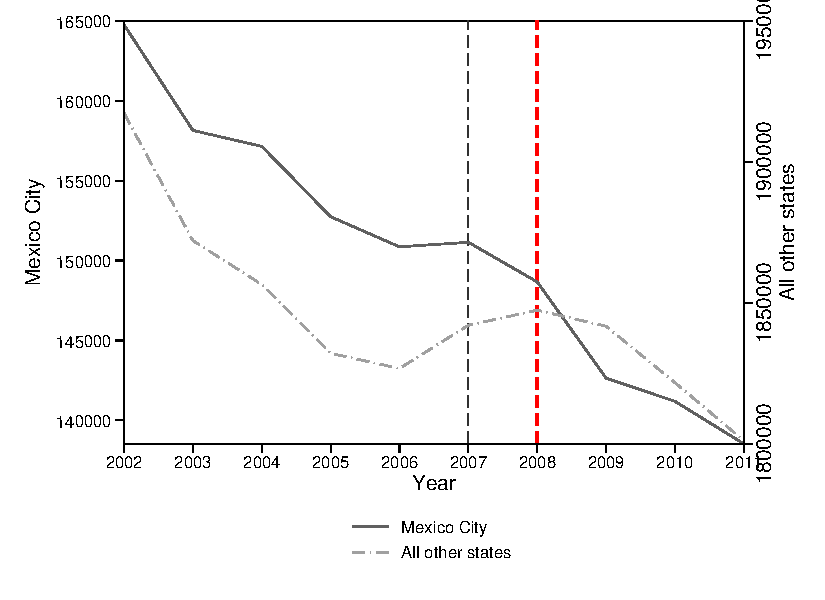
\includegraphics[scale=0.55]{../output/graphs/Trend_birth.pdf}
		\caption{Trends in Birth Rates}
		\label{ }
	\end{subfigure}%
	\begin{subfigure}{.5\textwidth}
		\centering
		\includegraphics[scale=0.55]{../output/graphs/Trend_mmr.pdf}
		\caption{Trends in Maternal Mortality Ratio}
		\label{ }
	\end{subfigure}
	\caption{Trends in Reform and non-Reform Areas}
	\label{ }
	\floatfoot{Note to figure \ref{trends}: Each figure is constructed from 
		administrative data made available by INEGI.  Trends are constructed based 
		on population weighted means for all fertile aged women.  The vertical 
		dashed line represents the date of the reform (for MMR), or 9 months
		following the date of the reform (for births) to account for the delay in
		the realisation of births due to gestation.}
\end{figure}

\input{../Results/Summary/Summary.tex}

\section*{Tables}
\begin{table}[htpb!]\caption{Main Regression}\label{reg1}
\begin{threeparttable}
	  \input{../output/regression/MainOutcomeMedPaper1.tex}
	\begin{tablenotes}
		\footnotesize
		\item \textit{Notes}.  The table displays the difference in difference estimates from OLS regressions. The sample includes all births for women aged 15-44 for the period 2002-2011. The dependent variables 1: \textit{Birth Rate} is defined as the annual number of births per 1000 women for each age group and state of birth. 2: The dependent variable \textit{Maternal Mortality Rate} refers to the annual number of maternal deaths per 100,000 live births for each age and state. The independent variable \textit{Reform} takes the value of one in locations and time where the reform was passed i.e. in the Federal District after 2007. The independent variable \textit{ReformClose} is a binary variable equal to one, post 2007, in the state of Mexico which is the surrounding district of the Federal District. State specific time trends are included. Standard errors (in parenthesis) are clustered at state level.*** p<0.01,** p<0.05,* p<0.1
	\end{tablenotes} 
\end{threeparttable}
\end{table}
 
 
 
\begin{table}[htpb!]\caption{Heterogenous effects across ages} \label{heteromed}
	\begin{threeparttable}
		
		{\small  \input{../output/regression/HetroEffectsMed.tex}}
		\begin{tablenotes}
			\footnotesize
			\item \textit{Notes}.  See notes of Table 2 and 3. The table shows the difference-in-difference estimates of the effect of the refrom on (a) birth rates (b) and maternal mortality by age group (15-19, 20-34, 35-39, and 40-44).
		\end{tablenotes} 
	\end{threeparttable}
\end{table}


 	
 	 

 


\end{spacing}

 % % % % % % % % % % % % % % % % % % % % % % % % % % %
 % % % % References % % % % % % % % % % % % % % % % % 
 % % % % % % % % % % % % % % % % % % % % % % % % % % %
 
 \newpage
 \singlespacing
 \bibliographystyle{agsm}
 \bibliography{bibfile}
 
 \newpage
\begin{appendices}
\section{Statistical Appendix}
 	We estimate the follwing specification:
 	\paragraph{specification 1}
 	
 	
 	\begin{eqnarray*}\label{eq1}
 		{Outcome_{ast}= \beta Reform_{st} +\beta ReformClose_{st}+} \\  
 		{	X_{st}\delta +\alpha_{s} + \nu_{t} +\pi_{a}+ \lambda_{s}*time_{t} +\epsilon_{ast}}   
 	\end{eqnarray*}
 	
 	\noindent where $Outcome_{ast}$ represents the outcome variables; birth rate, log transformed number of births, maternal mortality rate and log transformed number of maternal deaths for age $a$ in state $s$ and year $t$. Treatment status is indicated by $Reform$, which takes the value of 1 in locations and time where the reform was passed. The fixed effects are; state dummies $\alpha_{m}$, year dummies  $\nu_{t}$ and age dummies $\pi_{a}$. $X_{st}$ represents state-level time varying controls such as total output, subsidies, goods produced, number of public workers the roll out of the national health insurance program Seguro Popular.$\gamma_{s}$ is state-specific time trends. The idiosyncratic error term is denoted $\varepsilon_{ast}$ and clustered on state  level.

\section{Data Appendix}
Mexico: \citet{Aguirre1997,Walkeretal2004,Schiavonetal2012}

General: Measurement of MMR \citet{Hilletal2007,RonsmansGraham2006,Yazbeck2007}

Morbidity (?) \citet{Adleretal2012}

\section{Results Appendix}
 	
 	  \begin{figure}[htpb!]
 	  	\centering	\caption{Placebo tests}
 	  	\label{reg2}
 	  	\begin{subfigure}{.5\textwidth}
 	  		\centering	\caption{Birth Rates}
 	  		\includegraphics[scale=0.55]{../output/graphs/PlacebobirthRate.pdf}
 	  		
 	  		\label{placebo_br}
 	  	\end{subfigure}%
 	  	\begin{subfigure}{.5\textwidth}
 	  		\centering	\caption{Maternal Mortality Ratio}
 	  		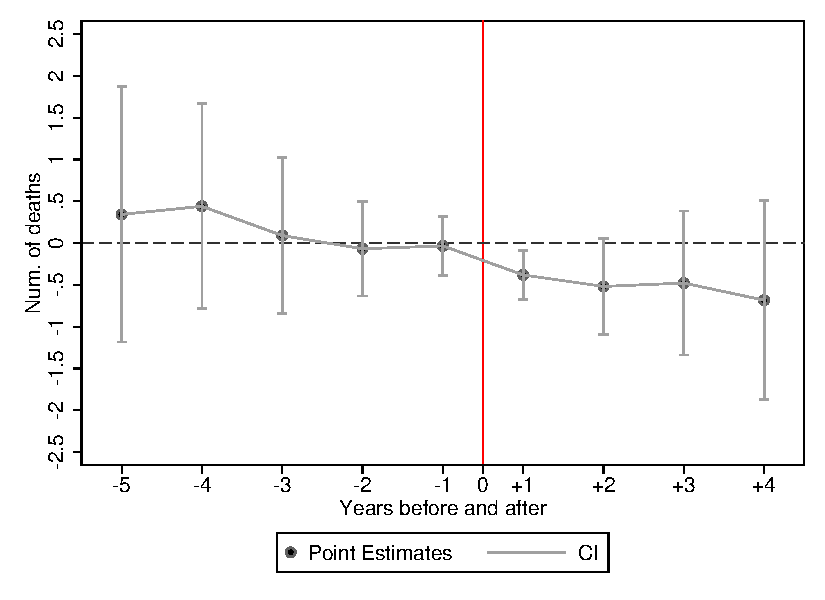
\includegraphics[scale=0.55]{../output/graphs/Placebommr.pdf}
 	  		
 	  		\label{placebo_mmr}
 	  	\end{subfigure}
 	  	\floatfoot{Note to figure ~\ref{reg2}: The coefficient plot shows specification 1 (without controlling for time varying factors), but instead of the using the Reform variable, leads and lags 4 years before and after the refrom are included in order to examine anticipatory effects as well as post treatment effects for birth rate (a) and maternal mortality (b) respectively.}
 	  \end{figure}

  \begin{figure}[htpb!]
  	\centering
  	\begin{subfigure}{.5\textwidth}
  		\centering
  		\includegraphics[scale=0.55]{../output/graphs/Trend_birthRate.pdf}
  		\caption{Trends in Birth Rates}
  		\label{birthTrend}
  	\end{subfigure}%
  	\begin{subfigure}{.5\textwidth}
  		\centering
  		\includegraphics[scale=0.55]{../output/graphs/Trend_mmr.pdf}
  		\caption{Trends in Maternal Mortality Ratio}
  		\label{mmrTrend}
  	\end{subfigure}
  	\caption{Trends in Reform and non-Reform Areas}
  	\label{trends}
  	\floatfoot{Note to figure \ref{trends}: Each figure is constructed from 
  		administrative data made available by INEGI.  Trends are constructed based 
  		on population weighted means for all fertile aged women.  The vertical 
  		dashed line represents the date of the reform (for MMR), or 9 months
  		following the date of the reform (for births) to account for the delay in
  		the realisation of births due to gestation.}
  \end{figure}	
  
  
  \begin{figure}[htpb!]
  	\centering	\caption{Trends in Reform and non-Reform Areas}
  	\label{trendsAge}
  	\begin{subfigure}{.5\textwidth}
  		\centering 
  		\includegraphics[scale=0.55]{../output/graphs/age.pdf}\caption{Trends in Maternal Age}
  		\label{age}
  	\end{subfigure}%
  	\begin{subfigure}{.5\textwidth}
  		\centering 	
  		\includegraphics[scale=0.55]{../output/graphs/EDAD_PADN.pdf}
  		\caption{Trends in Maternal Age}
  		\label{agedad}
  	\end{subfigure}
  	\begin{subfigure}{.5\textwidth}
  		\centering 
  		\includegraphics[scale=0.55]{../output/graphs/ageFirstChild.pdf}
  		\caption{Trends in Maternal Age at First Child}
  		\label{firstchild_mom}
  	\end{subfigure}%
  	\begin{subfigure}{.5\textwidth}
  		\centering
  		\includegraphics[scale=0.55]{../output/graphs/ageFirstChildDad.pdf}
  		\caption{Trends in Paternal Age at First Child}
  		\label{firstchild_dad}
  	\end{subfigure}
  	
  	\floatfoot{Note to figure \ref{age}: Each figure is constructed from 
  		administrative data made available by INEGI.}
  \end{figure}
  
   
   \begin{figure}[H] \caption{Synthetic Control Group} \centering
   	
   	\begin{subfigure}{.5\textwidth}
   		\centering 
   		\includegraphics[scale=0.55]{../output/graphs/synth.pdf}
   		\caption{MMR}
   	
   	\end{subfigure}%
   	\begin{subfigure}{.5\textwidth}
   		\centering
   		\includegraphics[scale=0.55]{../output/graphs/synthBR.pdf}
   		\caption{Birth Rate}
   		
   	\end{subfigure}
   	
    
   \end{figure} 
   
  \begin{figure}[htpb!]
  	\centering	\caption{Distribution of maternal age and age at first birth before and after the refrom}
  	\label{trendsAge}
  	\begin{subfigure}{.5\textwidth}
  		\centering 
  		\includegraphics[scale=0.55]{../output/graphs/HistAgeDF.pdf}\caption{Age in Mexico City}
  		\label{age}
  	\end{subfigure}%
  	\begin{subfigure}{.5\textwidth}
  		\centering 	
  		\includegraphics[scale=0.55]{../output/graphs/HistAgeOS.pdf}
  		\caption{Age in all other states}
  		\label{agedad}
  	\end{subfigure}
  	\begin{subfigure}{.5\textwidth}
  		\centering 
  		\includegraphics[scale=0.55]{../output/graphs/HistAgeFirstDF.pdf}
  		\caption{Age at first birth in Mexico City}
  		\label{firstchild_mom}
  	\end{subfigure}%
  	\begin{subfigure}{.5\textwidth}
  		\centering
  		\includegraphics[scale=0.55]{../output/graphs/HistAgeOS.pdf}
  		\caption{Age at first birth in all other states}
  		\label{firstchild_dad}
  	\end{subfigure}
  	
  	\floatfoot{Note to figure \ref{age}: Each figure is constructed from 
  		administrative data made available by INEGI.}
  \end{figure}
 	
 \end{appendices}
 
 



\end{document}
























%%%%%%%%%%%%%%%%%%%%%%%%%%%%%%%%%%%%%%%%%%%%%%%%%%%%%%%%%%%%%%%%%%%%%%%%%%%%%%%%%%%%%%%%%%
%%%%%%%%%%%%%%%%%%%%%%%%%%%%%%%%%%%%%%%%%%%%%%%%%%%%%%%%%%%%%%%%%%%%%%%%%%%%%%%%%%%%%%%%%%
%%%%%%%%%%%%%%%%%%%%%%%%%%%%%%%%%%%%%%%%%%%%%%%%%%%%%%%%%%%%%%%%%%%%%%%%%%%%%%%%%%%%%%%%%%
%%%%%%%%%%%%%%%%%%%%%%%%%%%%%%%%%%%%%%%%%%%%%%%%%%%%%%%%%%%%%%%%%%%%%%%%%%%%%%%%%%%%%%%%%%
%%%%%%%%%%%%%%%%%%%%%%%%%%%%%%%%%%%%%%%%%%%%%%%%%%%%%%%%%%%%%%%%%%%%%%%%%%%%%%%%%%%%%%%%%%
%%%%%%%%%%%%%%%%%%%%%%%%%%%%%%%%%%%%%%%%%%%%%%%%%%%%%%%%%%%%%%%%%%%%%%%%%%%%%%%%%%%%%%%%%%
%%%%%%%%%%%%%%%%%%%%%%%%%%%%%%%%%%%%%%%%%%%%%%%%%%%%%%%%%%%%%%%%%%%%%%%%%%%%%%%%%%%%%%%%%%
%%%%%%%%%%%%%%%%%%%%%%%%%%%%%%%%%%%%%%%%%%%%%%%%%%%%%%%%%%%%%%%%%%%%%%%%%%%%%%%%%%%%%%%%%%
%%%%%%%%%%%%%%%%%%%%%%%%%%%%%%%%%%%%%%%%%%%%%%%%%%%%%%%%%%%%%%%%%%%%%%%%%%%%%%%%%%%%%%%%%%
%%%%%%%%%%%%%%%%%%%%%%%%%%%%%%%%%%%%%%%%%%%%%%%%%%%%%%%%%%%%%%%%%%%%%%%%%%%%%%%%%%%%%%%%%%
%%%%%%%%%%%%%%%%%%%%%%%%%%%%%%%%%%%%%%%%%%%%%%%%%%%%%%%%%%%%%%%%%%%%%%%%%%%%%%%%%%%%%%%%%%
%%%%%%%%%%%%%%%%%%%%%%%%%%%%%%%%%%%%%%%%%%%%%%%%%%%%%%%%%%%%%%%%%%%%%%%%%%%%%%%%%%%%%%%%%%
%%%%%%%%%%%%%%%%%%%%%%%%%%%%%%%%%%%%%%%%%%%%%%%%%%%%%%%%%%%%%%%%%%%%%%%%%%%%%%%%%%%%%%%%%%
%%%%%%%%%%%%%%%%%%%%%%%%%%%%%%%%%%%%%%%%%%%%%%%%%%%%%%%%%%%%%%%%%%%%%%%%%%%%%%%%%%%%%%%%%%
%%%%%%%%%%%%%%%%%%%%%%%%%%%%%%%%%%%%%%%%%%%%%%%%%%%%%%%%%%%%%%%%%%%%%%%%%%%%%%%%%%%%%%%%%%
